\documentclass[11pt]{article}
\pdftrailerid{}
\usepackage[T1]{fontenc}
\usepackage{lmodern}
\pdfglyphtounicode{parenleftbig}{0028 FE01}
\pdfglyphtounicode{parenrightbig}{0029 FE01}
\pdfglyphtounicode{bracketleftbig}{005B FE01}
\pdfglyphtounicode{bracketrightbig}{005D FE01}
\pdfglyphtounicode{parenleftbigg}{0028 FE03}
\pdfglyphtounicode{parenrightbigg}{0029 FE03}
\pdfglyphtounicode{parenleftBigg}{0028 FE04}
\pdfglyphtounicode{parenrightBigg}{0029 FE04}
\pdfglyphtounicode{braceleftBigg}{007B FE04}
\pdfglyphtounicode{circleplusdisplay}{2A01 FE02}
\pdfglyphtounicode{summationtext}{2211 FE01}
\pdfglyphtounicode{producttext}{220F FE01}
\pdfglyphtounicode{summationdisplay}{2211 FE02}
\pdfglyphtounicode{integraldisplay}{222B FE02}
\pdfglyphtounicode{hatwide}{02C6 FE01}
\pdfglyphtounicode{ceilingleftBig}{2308 FE02}
\pdfglyphtounicode{ceilingrightBig}{2309 FE02}
\pdfglyphtounicode{braceleftBig}{007B FE02}
\pdfglyphtounicode{bracerightBig}{007D FE02}
\pdfglyphtounicode{radicalBig}{221A FE02}
\pdfglyphtounicode{productdisplay}{220F FE02}
\pdfglyphtounicode{hatwider}{02C6 FE02}
\pdfgentounicode=1
\usepackage[margin=1.05in]{geometry}
\usepackage{amsmath,amssymb,amsthm}
\usepackage{microtype}
\usepackage{needspace}
\usepackage{tikz}
\usepackage[hidelinks]{hyperref}

\newtheorem{theorem}{Theorem}
\newtheorem{lemma}[theorem]{Lemma}
\newtheorem{corollary}[theorem]{Corollary}
\newcommand{\E}{\mathbb E}
\newcommand{\Prb}{\mathbb P}
\newcommand{\Id}{\mathrm{Id}}
\newcommand{\HS}{\mathrm{HS}}
\newcommand{\op}{\mathrm{op}}
\newcommand{\sgn}{\operatorname{sgn}}
\newcommand{\norm}[1]{\lVert #1\rVert}
\newcommand{\abs}[1]{\lvert #1\rvert}
\newcommand{\ip}[2]{\langle #1,#2\rangle}

\hypersetup{
  pdftitle={Average sensitivity of polynomial threshold functions},
  pdfauthor={OpenAI},
  pdfsubject={Polynomial threshold functions and total influence on the Boolean cube},
  pdfkeywords={polynomial threshold function, average sensitivity, total influence, Boolean cube}
}
\urlstyle{same}
\title{Average sensitivity of polynomial threshold functions}
\author{OpenAI}
\date{September 25, 2026}

\begin{document}
\maketitle
\begin{abstract}
For every $n\ge1$ and $1\le d\le n$, we prove that a polynomial
threshold function of degree at most $d$ on the uniform Boolean cube has
average sensitivity at most $8d\sqrt n$. This proves the asymptotic form
of the Gotsman--Linial conjecture. The bound is uniform in both parameters
and uses the convention $\sgn(0)=1$.
\end{abstract}

\section{Introduction}\label{sec:introduction}

A polynomial threshold function assigns a sign to each vertex of the
Boolean cube by evaluating a real polynomial. On the cube, the identities
$x_i^2=1$ allow every polynomial to be replaced by a multilinear polynomial
of no larger degree without changing its values. Average sensitivity
measures the expected number of coordinate changes that reverse that sign.
For $x\in\{-1,1\}^n$, let $x^{\oplus i}$ be obtained by reversing
coordinate $i$. For $f:\{-1,1\}^n\to\{-1,1\}$, define
\begin{equation}\label{eq:influence-definition}
 I(f)=\sum_{i=1}^n\Prb\{f(X)\ne f(X^{\oplus i})\},
 \qquad X\text{ uniform on }\{-1,1\}^n.
\end{equation}
This quantity is also called the total influence of $f$. Throughout,
\[
 \sgn(t)=\begin{cases}1,&t\ge0,\\-1,&t<0.\end{cases}
\]
We prove the following estimate.

\begin{theorem}\label{thm:main}
Let $n\ge1$ and $1\le d\le n$ be integers. Let $p$ be a real multilinear
polynomial of degree at most $d$, and define
$f:\{-1,1\}^n\to\{-1,1\}$ by $f(x)=\sgn(p(x))$, with $\sgn(0)=1$.
Then, for average sensitivity under the uniform law,
\[
 I(f)\le 8d\sqrt n.
\]
\end{theorem}

The constant is independent of both $d$ and $n$. In particular, the degree
may grow with the dimension. The polynomial may vanish on the cube, and
no regularity condition is imposed on $p$.

Gotsman and Linial proposed an exact extremal bound for average
sensitivity~\cite[Section~5, p.~47]{GotsmanLinial1994}.
Their candidate is symmetric: it is the sign of a degree-$d$ polynomial
in $x_1+\cdots+x_n$ whose roots lie between the central levels of the
cube. The proposal asserts that this function maximizes influence among
all degree-$d$ polynomial threshold functions in $n$ variables.
Chapman constructed counterexamples to this exact assertion and
explicitly distinguished it from the asymptotic bound
$I(f)=O(d\sqrt n)$
\cite[Conjectures~1.1--1.2 and Theorem~1.1]{Chapman2018}.
Kim, Maldonado, and Wellens independently constructed quadratic
counterexamples for odd $n\ge5$ and proved influence bounds for
quadratic polynomials with restricted support
graphs~\cite[Theorems~1.1--1.3]{KimMaldonadoWellens2017}.
Theorem~\ref{thm:main} establishes the asymptotic bound with an absolute
constant; it makes no assertion about exact maximizers.
Numbered locators in references with a listed preprint refer to that
preprint version.

The classical symmetric examples explain the scale of the theorem.
Let $1\le d\le\sqrt n$, let $J$ consist of the $d$ indices nearest
$(n-1)/2$ in $\{0,\ldots,n-1\}$, breaking a tie arbitrarily, and put
\[
 t(x)=\frac{n+x_1+\cdots+x_n}{2},\qquad
 p_J(x)=\prod_{j\in J}\bigl(t(x)-j-\tfrac12\bigr).
\]
Here $t(x)$ is the number of coordinates of $x$ equal to $+1$.
Multilinearization preserves the values of $p_J$ on the cube and has
degree at most $d$. Its sign changes exactly across the boundaries
between Hamming weights $j$ and $j+1$ for $j\in J$. There are
$(n-j)\binom nj=n\binom{n-1}j$ unoriented edges at such a boundary,
so the ordered-edge normalization in~\eqref{eq:influence-definition}
gives
\[
 I(\sgn p_J)=n\,2^{-(n-1)}\sum_{j\in J}\binom{n-1}j
 \asymp d\sqrt n.
\]
Here the comparison constants are absolute. The central-binomial
estimate from Stirling's formula, together with the ratios of consecutive
binomial coefficients, shows that the binomial masses are comparable
to $n^{-1/2}$ within $\sqrt n/2$ of the center, which includes all
selected indices; the case $n=1$ follows directly from the count.
Thus the order $d\sqrt n$ is sharp throughout
this degree range; see also
\cite[p.~3, discussion following Theorem~1.1]{KimMaldonadoWellens2017}.
For every Boolean function, the additional bound $I(f)\le n$ holds.

Early general bounds established sublinear influence for every fixed
degree. For $n>1$, Harsha, Klivans, and Meka proved
$I(f)\le2^{O(d)}n^{1-1/(4d+6)}$
\cite[Theorem~1.6]{HarshaKlivansMeka2014}, while the independent work of
Diakonikolas, Raghavendra, Servedio, and Tan gave
$I(f)\le2^{O(d)}(\log n)n^{1-1/(4d+2)}$
\cite[Theorem~1.1]{DRST2014}.
These results first circulated in 2009, before their 2014 journal
publications. Their proofs use regularity and invariance arguments to
compare sufficiently regular Boolean polynomials with Gaussian ones.
Kane subsequently established the square-root exponent in the dimension:
\begin{equation}\label{eq:kane-bound}
 I(f)\le\sqrt n\,(\log n)^{O(d\log d)}2^{O(d^2\log d)}
 \qquad(n>1)
\end{equation}
\cite[Theorem~2]{Kane2014}.
For each fixed $d\ge2$, this is an $n^{1/2+o(1)}$ bound with a
polylogarithmic loss. His proof combines random restrictions, regularity,
and invariance estimates. Theorem~\ref{thm:main} removes that loss and
gives linear dependence on $d$ with an absolute constant.

Small moments of the local sensitivity
$s_f(x)=|\{i:f(x)\ne f(x^{\oplus i})\}|$ give further information
about its distribution. Chang, Slote, Volberg, and Zhang bounded the
Boolean surface area $\E\sqrt{s_f(X)}$ by a polynomial in $\log(en)$
for each fixed degree
\cite[Theorem~1.1, equation~(1.6)]{ChangSloteVolbergZhang2026}.
Tseng and Volberg studied a wider range of sensitivity moments
\cite{TsengVolberg2026}.
For comparison with the first moment, the pointwise inequality
$s_f\le\sqrt n\sqrt{s_f}$ converts the surface-area estimate into an
influence bound with a logarithmic loss. At moment order one, the
estimate in~\cite[Section~2.5, equation~(11)]{TsengVolberg2026}
is $C(d)\sqrt n(\log n)^{Cd\log d}$ for $n>1$, which likewise retains a
logarithmic factor for $d\ge2$.

\paragraph{Proof strategy.}
The proof separates a probability estimate from a finite-dimensional
operator construction. The probability estimate says that equal-law
random variables of variance $\sigma^2$ satisfy
$\E(U-V)^2\le8a\sigma$ whenever $V-U\le a$ almost surely.
A bound on increments in the opposite direction is not assumed.
Equality of the marginal laws supplies the needed balance through an
increasing function whose increments dominate squared displacement.
Section~\ref{sec:coupling} proves this estimate directly.

For the operator construction, begin with the spaces of cube polynomials
of degrees at most $k$, for $0\le k\le n$. Multiply these spaces by
$\sqrt w$ for a positive weight $w$, and take their successive orthogonal
increments in the counting inner product. The increments have dimensions
$\binom nk$, although the weight changes their positions. Give the
$k$th increment eigenvalue $k-n/2$; this defines a self-adjoint operator
$M$ with fixed squared Hilbert--Schmidt norm $n2^n/4$.
Its squared Hilbert--Schmidt norm is the sum of the squared moduli of
all matrix entries.
Multiplication by a coordinate connects only equal or adjacent grades,
because it raises polynomial degree by at most one and is self-adjoint.
These are the two features of the grading used in the proof: fixed
dimensions and locality under coordinate multiplication
(Section~\ref{sec:grading}).

When $w\equiv1$, $M$ is minus one-half of the cube adjacency matrix.
For a general weight, some edge entries may have smaller squared modulus,
and other entries may appear. Section~\ref{sec:edges} shows that the total squared
entry mass between vertices at distance at least two is bounded by the
mass on the diagonal.
Together with a bound on each edge entry, this controls the total deficit
from the unweighted squared edge value $1/4$.
If $H$ multiplies by a sign function $h$, the anticommutator $MH+HM$
retains diagonal entries and equal-sign edge entries, multiplying them by
$2$ or $-2$. Its squared norm therefore bounds the number of equal-sign
edges even for an arbitrary positive weight.

Finally, multiply $f$ by full parity to obtain
$h(x)=(\prod_{i=1}^n x_i)f(x)$, and use $w=|p|$ after removing zeros
without changing signs. The equal-sign edges of $h$ are exactly the
sensitive edges of $f$. Moreover, multiplication by parity turns the
Fourier support of $p$ into degrees at least $n-d$.
This forces the block of $H$ between grades $r$ and $s$ to vanish when
$r+s<n-d$. The normalized squared block norms define a probability law
for $(R,S)$ whose two marginals are $\operatorname{Bin}(n,1/2)$.
Reflecting one index gives $U=S$ and $V=n-R$, with the same marginals and
$V-U\le d$. The coupling estimate then bounds the anticommutator norm,
and the edge estimate gives the theorem. Section~\ref{sec:parity}
performs this assembly, keeping track of ordered edges.

\paragraph{Consequences.}
Section~\ref{sec:consequences} derives a dimension-free Boolean noise
sensitivity bound and a quantitative learning guarantee from the influence
estimate. The learning statement concerns independent labeled samples
whose input marginal is uniform, while the labels may be arbitrary.
It follows by combining noise smoothing with polynomial regression.

\section{A one-sided coupling estimate}\label{sec:coupling}

The next lemma controls mean square displacement from an upper bound in
only one direction. Large downward displacements are permitted, so
bounding the positive and negative displacements separately would lose
information. Equality of the marginal laws instead balances the expected
change of any integrable function applied to the two variables. We use
an increasing function whose increments dominate squared displacement;
its increments in the bounded direction can be estimated using the common
variance. Neither independence nor exchangeability is assumed.

\Needspace{5\baselineskip}
\begin{lemma}\label{lem:coupling}
Let $U,V$ be real random variables with the same distribution, finite mean
$m$, and finite variance $\sigma^2$. If $V-U\le a$ almost surely, where
$a\ge0$, then
\[
 \E(U-V)^2\le 8a\sigma.
\]
\end{lemma}

\begin{proof}
The function $|t-m|$ grows linearly away from the common mean. Its
primitive is the increasing function
\[
 g(t)=\int_m^t\abs{z-m}\,dz=\tfrac12(t-m)\abs{t-m}.
\]
For $u<v$, we have
\begin{equation}\label{eq:g-increments}
 \frac{(v-u)^2}{4}\le g(v)-g(u)
 \le \frac{v-u}{2}\bigl(\abs{u-m}+\abs{v-m}\bigr).
\end{equation}
For the lower bound, if $u\le m\le v$, the integral is
$\bigl((m-u)^2+(v-m)^2\bigr)/2\ge(v-u)^2/4$; if the interval lies on one
side of $m$, the integral is at least $(v-u)^2/2$.
For the upper bound, convexity places $\abs{z-m}$ below the chord joining
its endpoint values, whose integral is the displayed upper bound.

The second-moment assumption makes $g(U)$ and $g(V)$ integrable.
Their expectations agree. For the integrable random variable
$Y=g(V)-g(U)$, write $Y_+=\max\{Y,0\}$. The identity $\E Y=0$ implies
$\E|Y|=2\E Y_+$. Since $g$ is strictly increasing, $Y>0$ exactly when
$V>U$, and hence
\begin{align*}
 \E\abs{g(U)-g(V)}
 &=2\E\bigl[\mathbf1_{\{V>U\}}(g(V)-g(U))\bigr]\\
 &\le a\E\bigl[\abs{U-m}+\abs{V-m}\bigr]
 \le 2a\sigma.
\end{align*}
The first inequality uses \eqref{eq:g-increments} and $V-U\le a$ on
$\{V>U\}$; the last is Cauchy--Schwarz.
The lower bound in \eqref{eq:g-increments}, with the endpoints put in
increasing order, gives $(U-V)^2\le4|g(U)-g(V)|$ pointwise. Taking
expectations proves the lemma.
\end{proof}


The cancellation $\E[g(V)-g(U)]=0$ uses only equality of marginal laws.
Primitive differences with this property also appear in R\"ollin's
formulation of Stein's method~\cite[Section~1]{Rollin2008}.
The present one-sided second-moment estimate follows from the elementary
increment bounds above.

\section{Weighted Fourier grading}\label{sec:grading}

We next construct an operator whose spectrum is fixed by the dimensions
of polynomial spaces, while its matrix entries respond to an arbitrary
positive weight. The construction is the cube instance of the usual degree
filtration for discrete multivariate orthogonal polynomials, whose
coordinate multipliers satisfy a three-term recurrence; compare
Xu~\cite[Section~3]{Xu2004}. We give the finite-dimensional argument in
the present notation.


Write $\Omega=\{-1,1\}^n$ and $N=2^n$. We work in
$\mathcal H=\mathbb C^\Omega$ with the counting inner product
\[
 \ip{a}{b}=\sum_{x\in\Omega}\overline{a(x)}b(x).
\]
Thus the point masses $\delta_x$ form an orthonormal basis. For an operator
$B$, write $B_{xy}=\ip{\delta_x}{B\delta_y}$ and let
\[
 \norm B_{\HS}^2=\sum_{x,y\in\Omega}\abs{B_{xy}}^2
\]
be its Hilbert--Schmidt norm squared; $\norm B_{\op}$ denotes its operator
norm. The Hilbert--Schmidt norm is independent of the orthonormal basis.

For $S\subseteq[n]=\{1,\ldots,n\}$, set
$\chi_S(x)=\prod_{j\in S}x_j$. These real characters satisfy
\[
 \ip{\chi_S}{\chi_T}=N\mathbf1_{\{S=T\}},\qquad
 \chi_S\chi_T=\chi_{S\mathbin\triangle T}.
\]
Indeed, a nonconstant character sums to zero by pairing vertices that
differ in one of its coordinates. The displayed product rule therefore
gives orthogonality, and the $N$ characters form a basis of the
$N$-dimensional space $\mathcal H$. Let
\[
 V_k=\operatorname{span}\{\chi_S:\abs S\le k\},\qquad 0\le k\le n,
\]
and set $V_k=\mathcal H$ for $k\ge n$. Membership in $V_k$ means that a
function has Fourier degree at most $k$. The character multiplication rule
shows that $a\in V_r$ and $b\in V_s$ imply $\overline b a\in V_{r+s}$.

Fix any function $w:\Omega\to(0,\infty)$, and let $D$ be multiplication
by $\sqrt w$. The identity
\[
 \ip{Da}{Db}=\sum_{x\in\Omega}w(x)\overline{a(x)}b(x)
\]
identifies the weighted inner product with the counting inner product
after applying $D$. We can therefore orthogonalize polynomial degrees for the weight
$w$ while retaining the orthonormal point basis used to count edges.
Form the nested subspaces
\[
 K_k=DV_k,\qquad K_{-1}=\{0\},\qquad
 E_k=K_k\cap K_{k-1}^{\perp}\quad(0\le k\le n).
\]
Let $\Pi_k$ be the orthogonal projection onto $E_k$. The spaces $K_k$
are nested, and $K_k=K_{k-1}\oplus E_k$. Since $D$ is invertible,
$\dim K_k=\dim V_k=\sum_{j=0}^k\binom nj$ and $K_n=\mathcal H$.
Subtracting consecutive dimensions gives
\[
\mathcal H=\bigoplus_{k=0}^n E_k,\qquad
 \dim E_k=\binom nk.
\]
Choosing an orthonormal basis in each $E_k$ and decomposing the image of
each basis vector gives, for every operator $B$,
\begin{equation}\label{eq:block-parseval}
 \norm B_{\HS}^2
 =\sum_{r,s=0}^n\norm{\Pi_s B\Pi_r}_{\HS}^2.
\end{equation}
Define the grading operator and its centered version by
\begin{equation}\label{eq:grading}
 L=\sum_{k=0}^n k\Pi_k,\qquad M=L-\frac n2\Id.
\end{equation}
They are self-adjoint. Their prescribed eigenvalue multiplicities give
\begin{equation}\label{eq:total-energy}
 \norm M_{\HS}^2=\sum_{k=0}^n\binom nk\left(k-\frac n2\right)^2
 =\frac{nN}{4}.
\end{equation}
The last equality is the variance identity for a sum of $n$ independent
Bernoulli random variables of parameter $1/2$.

Let $\rho(x,y)$ denote Hamming distance. All pairs of vertices in what
follows are \emph{ordered}. When $w\equiv1$, the identity
$\sum_{y:\rho(x,y)=1}\chi_S(y)=(n-2\abs S)\chi_S(x)$ shows that $M$ is
minus one-half of the cube adjacency matrix. Thus every edge entry has
squared modulus $1/4$; the proof below controls the total deficit from
this value for arbitrary positive weights.

The key local property is that multiplying by a coordinate connects
only equal or adjacent grades.

For each $i\in[n]$, let $Z_i$ be multiplication by $x_i$. It is a
self-adjoint unitary and commutes with $D$. Multiplication by $x_i$ raises
Fourier degree by at most one, so $Z_iK_r\subseteq K_{r+1}$.
For $s>r+1$, the inclusion $K_{r+1}\subseteq K_{s-1}$ and the
orthogonality $E_s\perp K_{s-1}$ give $\Pi_sZ_i\Pi_r=0$.
Taking adjoints gives the opposite triangular vanishing, so
\begin{equation}\label{eq:tridiagonal}
 \Pi_sZ_i\Pi_r=0\qquad\text{whenever }\abs{s-r}>1.
\end{equation}

Together with the fixed total energy in \eqref{eq:total-energy}, this
restriction will control the entries of $M$ between vertices at Hamming
distance at least two.

\section{Recovering edges from the anticommutator}\label{sec:edges}

Keep the grading of Section~\ref{sec:grading}, with no restriction on the
positive weight $w$. For an operator $H$ that multiplies by a sign, the
anticommutator $MH+HM$ vanishes between opposite signs and multiplies
entries of $M$ by $2$ or $-2$ between equal signs. The following lemma turns this observation into an edge
count even though an arbitrary weight can change the individual edge
entries.

\begin{lemma}[Recovering edges from the grading]\label{lem:edges}
Let $n\ge1$, $\Omega=\{-1,1\}^n$, and $w:\Omega\to(0,\infty)$.
Let $M$ be the centered grading operator \eqref{eq:grading} constructed
from $w$. For $h:\Omega\to\{-1,1\}$, let $H$ be multiplication by $h$
and set
\[
 \mathcal E_h=\{(x,y)\in\Omega^2:\rho(x,y)=1,\ h(x)=h(y)\}.
\]
Then, counting ordered pairs,
\begin{equation}\label{eq:edge-recovery}
 \abs{\mathcal E_h}\le 2\norm{MH+HM}_{\HS}^2.
\end{equation}
\end{lemma}

\begin{proof}
We compare $M$ with the unweighted grading, whose edge entries have
squared modulus $1/4$. First we show that every edge entry of $M$ has
squared modulus at most $1/4$. We then bound the sum of the deficits by
diagonal energy, which
the anticommutator detects for every choice of signs.

\smallskip\noindent\emph{A bound for each off-diagonal entry.}
Write $C_i=[L,Z_i]=[M,Z_i]$, where $[A,B]=AB-BA$.
Its grade blocks are
\[
 \Pi_sC_i\Pi_r=(s-r)\Pi_sZ_i\Pi_r.
\]
We will prove $\norm{C_i}_{\op}\le1$. The commutator keeps only
adjacent-grade blocks, with opposite signs in the two directions.
We first remove the equal-grade blocks by a norm-nonincreasing average,
then supply those opposite signs, up to a common phase, by unitary
conjugation. Introduce the unitaries
\[
 J=\sum_{k=0}^n(-1)^k\Pi_k,\qquad
 W=\sum_{k=0}^n\mathrm i^k\Pi_k,
 \qquad \mathrm i^2=-1.
\]
Set $O_i=(Z_i-JZ_iJ)/2$. The triangle inequality gives
$\norm{O_i}_{\op}\le(\norm{Z_i}_{\op}+\norm{JZ_iJ}_{\op})/2=1$.
In the $(s,r)$ block, the factor defining $O_i$ is
$(1-(-1)^{s+r})/2$. It is zero on the diagonal and one when
$|s-r|=1$. By \eqref{eq:tridiagonal}, $O_i$ therefore consists precisely
of the blocks of $Z_i$ with
$\abs{s-r}=1$. On these blocks, conjugation by $W$ multiplies by
$\mathrm i^{s-r}=\mathrm i(s-r)$. Therefore
\[
 WO_iW^*=\mathrm i C_i,
 \qquad\text{and hence}\qquad \norm{C_i}_{\op}\le1.
\]
In the point basis, $(C_i)_{xy}=(y_i-x_i)M_{xy}$.
If $x\ne y$, choose $i$ with $x_i\ne y_i$ to obtain
\[
 2\abs{M_{xy}}=\abs{(C_i)_{xy}}\le\norm{C_i}_{\op}\le1.
\]
In particular, each neighbor deficit $1/4-\abs{M_{xy}}^2$ is nonnegative.

\smallskip\noindent\emph{The total neighbor deficit.}
The same grade blocks also give an aggregate bound. By
\eqref{eq:block-parseval} and \eqref{eq:tridiagonal},
\[
 \norm{C_i}_{\HS}^2
 =\sum_{r,s=0}^n(s-r)^2\norm{\Pi_sZ_i\Pi_r}_{\HS}^2
 \le\norm{Z_i}_{\HS}^2=N.
\]
Summing the squared point-basis entries of $C_i$ over coordinates gives
\begin{equation}\label{eq:distance-energy}
 \sum_{x,y}\rho(x,y)\abs{M_{xy}}^2
 =\frac14\sum_{i=1}^n\norm{C_i}_{\HS}^2
 \le\frac{nN}{4}=\sum_{x,y}\abs{M_{xy}}^2,
\end{equation}
where the last equality is \eqref{eq:total-energy}. Set
\[
 A_0=\sum_x\abs{M_{xx}}^2,\qquad
 F=\sum_{\rho(x,y)\ge2}\abs{M_{xy}}^2.
\]
The difference between the outermost sums in
\eqref{eq:distance-energy} is
$-A_0+\sum_{\rho(x,y)\ge2}(\rho(x,y)-1)|M_{xy}|^2\le0$.
Thus energy beyond neighboring pairs is bounded by diagonal energy:
\begin{equation}\label{eq:far-energy}
 F\le\sum_{\rho(x,y)\ge2}(\rho(x,y)-1)\abs{M_{xy}}^2\le A_0.
\end{equation}

There are $nN$ ordered neighbor pairs, and thus
\begin{align}
 \sum_{\rho(x,y)=1}\left(\frac14-\abs{M_{xy}}^2\right)
 &=\frac{nN}{4}-\sum_{\rho(x,y)=1}\abs{M_{xy}}^2\notag\\
 &=A_0+F\le2A_0.\label{eq:deficit}
\end{align}
Here we used \eqref{eq:total-energy} and \eqref{eq:far-energy}.
The fixed total energy consequently controls the full deficit from the
unweighted edge value $1/4$.

\smallskip\noindent\emph{Recovering the equal-sign edges.}
Let $A_h=\sum_{(x,y)\in\mathcal E_h}\abs{M_{xy}}^2$.
Because the individual deficits are nonnegative, their sum over
$\mathcal E_h$ is at most the full sum in \eqref{eq:deficit}. Hence
\begin{equation}\label{eq:count-deficit}
 \frac{\abs{\mathcal E_h}}4\le A_h+2A_0\le2(A_h+A_0).
\end{equation}
For $T=MH+HM$ we have
$T_{xy}=(h(x)+h(y))M_{xy}$. On both the diagonal and $\mathcal E_h$,
the squared factor is $4$, so
\[
 4(A_0+A_h)\le\norm T_{\HS}^2.
\]
Together with \eqref{eq:count-deficit}, this proves
\eqref{eq:edge-recovery}.
\end{proof}

\section{Parity and the binomial coupling}\label{sec:parity}

We now choose the weight from the polynomial. Parity will convert the
sensitivity problem into the equal-sign edge count of
Lemma~\ref{lem:edges}, while the polynomial degree will produce the
one-sided constraint needed for Lemma~\ref{lem:coupling}.

\begin{proof}[Proof of Theorem~\ref{thm:main}]

We may assume that $p(x)\ne0$ for every $x\in\Omega$.
Indeed, if $p$ takes negative values, add a positive constant smaller than
$\min\{\abs{p(x)}:p(x)<0\}$; otherwise add any positive constant.
Negative values remain negative, while zero values become positive and
positive values stay positive. Thus the perturbation preserves $f$ under
our convention $\sgn(0)=1$, does not increase the degree, and makes $p$
nonzero at every vertex. We henceforth use $p$ for the perturbed polynomial.

Let $\chi=\chi_{[n]}$ be full parity and set
\[
 w=\abs p,\qquad h=\chi f,\qquad q=\chi p.
\]
Full parity changes sign across every edge, so $h(x)=h(y)$ for neighbors
$x,y$ exactly when $f(x)\ne f(y)$. Consequently
\begin{equation}\label{eq:sensitivity-count}
 I(f)=\frac{\abs{\mathcal E_h}}N.
\end{equation}
Here both sides count sensitive edges in both directions.
We have $w>0$ and $hw=q$. Construct the weighted grading
\eqref{eq:grading} from $w$, and let $H$ be multiplication by $h$.
Since $\chi\chi_S=\chi_{[n]\setminus S}$ and $\deg p\le d$, the Fourier
support of $q$ lies in degrees at least $n-d$.

We claim that
\begin{equation}\label{eq:vanishing}
 \Pi_sH\Pi_r=0\qquad\text{if }r+s<n-d.
\end{equation}
To see this, write elements of $E_r\subseteq DV_r$ and $E_s\subseteq DV_s$
as $Da$ and $Db$, with $a\in V_r$ and $b\in V_s$. Then
\[
 \ip{Db}{HDa}=\sum_{x\in\Omega}\overline{b(x)}a(x)w(x)h(x)
 =\sum_{x\in\Omega}\overline{b(x)}a(x)q(x)=0.
\]
The last equality follows from character orthogonality: the product
$\overline b a$ has Fourier degree at most $r+s<n-d$.

Set $T=MH+HM$. Its blocks are
\begin{equation}\label{eq:T-blocks}
 \Pi_sT\Pi_r=(s+r-n)\Pi_sH\Pi_r.
\end{equation}
Thus the anticommutator energy is a weighted second moment of the sum of
the two grade indices:
\[
 \frac1N\norm T_{\HS}^2
 =\sum_{r,s=0}^n(s+r-n)^2\,
   \frac{\norm{\Pi_sH\Pi_r}_{\HS}^2}{N}.
\]
The coefficients on the right define a probability distribution. Indeed,
because $H$ is unitary and the projections are orthogonal,
\[
 \sum_s\norm{\Pi_sH\Pi_r}_{\HS}^2
 =\norm{H\Pi_r}_{\HS}^2=\binom nr.
\]
Decomposing the domain into grades and taking adjoints likewise gives
\[
 \sum_r\norm{\Pi_sH\Pi_r}_{\HS}^2
 =\norm{\Pi_sH}_{\HS}^2
 =\norm{H^*\Pi_s}_{\HS}^2=\binom ns.
\]
Since $\sum_r\binom nr=N$, we may therefore define random indices
$R,S\in\{0,\ldots,n\}$ by
\begin{equation}\label{eq:block-coupling}
 \Prb\{R=r,S=s\}=\frac1N\norm{\Pi_sH\Pi_r}_{\HS}^2.
\end{equation}
Both marginals are $\operatorname{Bin}(n,1/2)$, and the preceding energy
identity becomes
\[
 \frac1N\norm T_{\HS}^2=\E(R+S-n)^2.
\]

To use Lemma~\ref{lem:coupling}, reflect the first index: put $U=S$ and
$V=n-R$. Binomial symmetry gives $U$ and $V$ the same distribution,
with mean $n/2$ and variance $n/4$. Meanwhile,
\eqref{eq:vanishing} gives $R+S\ge n-d$ almost surely, which becomes
$V-U\le d$. Figure~\ref{fig:grade-coupling} shows how the zero-block
region becomes this one-sided support constraint.

\begin{figure}[!htbp]
  \centering
  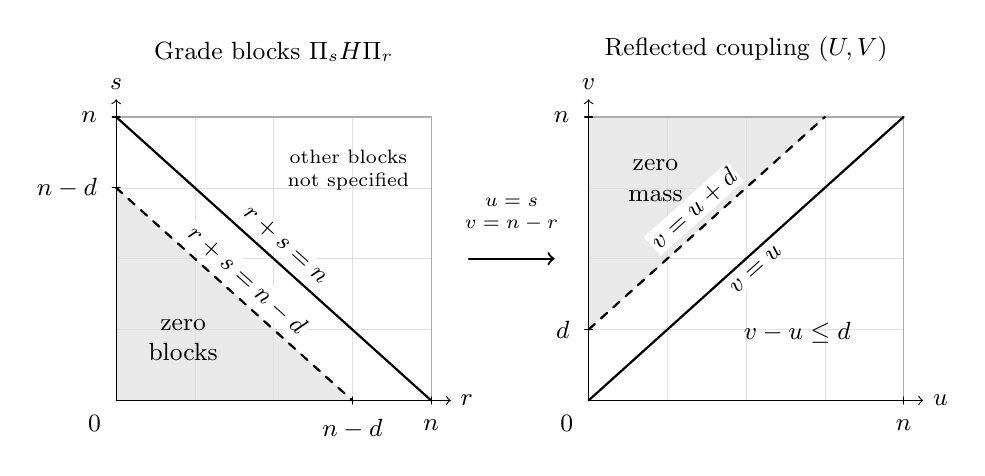
\begin{tikzpicture}[x=1cm,y=.9cm,line cap=round,line join=round,
                      font=\small]
    \begin{scope}
      \fill[gray!17] (0,0) -- (3,0) -- (0,3) -- cycle;
      \draw[step=1,gray!25,very thin] (0,0) grid (4,4);
      \draw[gray!65] (0,4) -- (4,4) -- (4,0);
      \draw[->] (0,0) -- (4.25,0) node[right] {$r$};
      \draw[->] (0,0) -- (0,4.25) node[above] {$s$};
      \node[below left=2pt] at (0,0) {$0$};
      \draw (3,.05) -- (3,-.05) node[below=2pt] {$n-d$};
      \draw (4,.05) -- (4,-.05) node[below=2pt] {$n$};
      \draw (.05,3) -- (-.05,3) node[left=2pt] {$n-d$};
      \draw (.05,4) -- (-.05,4) node[left=2pt] {$n$};
      \draw[thick,dashed] (0,3) -- (3,0)
        node[midway,above=2pt,sloped,fill=white,inner sep=1pt]
        {$r+s=n-d$};
      \draw[thick] (0,4) -- (4,0)
        node[midway,above=2pt,sloped,fill=white,inner sep=1pt]
        {$r+s=n$};
      \node[align=center] at (.85,.85) {zero\\blocks};
      \node[align=center,font=\scriptsize] at (2.95,3.25)
        {other blocks\\not specified};
      \node[above=10pt] at (2,4.25) {Grade blocks $\Pi_sH\Pi_r$};
    \end{scope}

    \draw[->,thick] (4.48,2) -- (5.57,2);
    \node[align=center,font=\scriptsize] at (5.02,2.63)
      {$u=s$\\$v=n-r$};

    \begin{scope}[xshift=6cm]
      \fill[gray!17] (0,1) -- (0,4) -- (3,4) -- cycle;
      \draw[step=1,gray!25,very thin] (0,0) grid (4,4);
      \draw[gray!65] (0,4) -- (4,4) -- (4,0);
      \draw[->] (0,0) -- (4.25,0) node[right] {$u$};
      \draw[->] (0,0) -- (0,4.25) node[above] {$v$};
      \node[below left=2pt] at (0,0) {$0$};
      \draw (4,.05) -- (4,-.05) node[below=2pt] {$n$};
      \draw (.05,1) -- (-.05,1) node[left=2pt] {$d$};
      \draw (.05,4) -- (-.05,4) node[left=2pt] {$n$};
      \draw[thick,dashed] (0,1) -- (3,4)
        node[midway,above=2pt,sloped,fill=white,inner sep=1pt]
        {$v=u+d$};
      \draw[thick] (0,0) -- (4,4)
        node[midway,below=2pt,sloped,fill=white,inner sep=1pt]
        {$v=u$};
      \node[align=center] at (.85,3.1) {zero\\mass};
      \node at (2.65,.95) {$v-u\le d$};
      \node[above=10pt] at (2,4.25) {Reflected coupling $(U,V)$};
    \end{scope}
  \end{tikzpicture}
  \[
    \mathbb P\{R=r,S=s\}
      =2^{-n}\|\Pi_sH\Pi_r\|_{\mathrm{HS}}^2,
    \qquad r+s-n=u-v.
  \]
  \caption{Grade blocks and their reflected coupling, schematic for $0<d<n$.
  Under $U=S$, $V=n-R$, the zero-block region $r+s<n-d$ becomes the
  zero-mass region $v-u>d$, giving $V-U\le d$ almost surely.
  Dashed boundaries are allowed; solid diagonals mark $r+s-n=u-v=0$.
  Each marginal is $\operatorname{Bin}(n,1/2)$. Unshaded locations need
  not carry positive mass, and grid spacing is illustrative.}
  \label{fig:grade-coupling}
\end{figure}


Apply Lemma~\ref{lem:coupling} with $a=d$ and $\sigma=\sqrt n/2$ to obtain
\begin{equation}\label{eq:coupling-bound}
 \frac1N\norm T_{\HS}^2
 =\E(R+S-n)^2=\E(U-V)^2\le4d\sqrt n.
\end{equation}
Finally, \eqref{eq:sensitivity-count} and Lemma~\ref{lem:edges} give
\[
 I(f)=\frac{\abs{\mathcal E_h}}N
 \le\frac2N\norm T_{\HS}^2
 \le8d\sqrt n.
\]
This completes the proof.
\end{proof}



\section{Noise sensitivity and agnostic learning}\label{sec:consequences}

The influence bound has two consequences that are independent of the
weighted grading used to prove it. A random-bucketing construction
transfers the bound from one-bit changes to independent noise.
Smoothing by this noise then gives low-degree polynomial approximants,
which yield an agnostic learner by $L_1$ regression.

\subsection{Noise sensitivity}

For $0\le\eta\le1/2$, define the noise sensitivity
$\operatorname{NS}_{\eta}(f)=\Prb\{f(X)\ne f(Y)\}$, where $X$ is uniform
on the cube and $Y$ is obtained by flipping each coordinate of $X$
independently with probability $\eta$.

\begin{corollary}[Boolean noise sensitivity]\label{cor:noise-sensitivity}
Let $n\ge1$ and $d\ge0$ be integers. If $f=\sgn(p)$ on
$\{-1,1\}^n$ for a real polynomial $p$ of degree at most $d$, with
$\sgn(0)=1$, then
\[
 \operatorname{NS}_{\eta}(f)\le C d\sqrt\eta
 \qquad(0<\eta\le1/2),
\]
where $C$ is an absolute constant.
\end{corollary}

\begin{proof}
Constants have zero noise sensitivity. For an integer $q\ge2$, use the
random-bucketing reduction of Diakonikolas, Raghavendra, Servedio, and
Tan~\cite[Section~7.1, equation~(14)]{DRST2014}: choose independent uniform
signs $a_i$ and independent uniform buckets $b(i)\in\{1,\ldots,q\}$,
and set
\[
 g(z)=f(a_1z_{b(1)},\ldots,a_nz_{b(n)}),
 \qquad z\in\{-1,1\}^q.
\]
Multilinearizing the substituted polynomial preserves its cube values,
including zeros, and gives degree at most $\min(d,q)$.
Theorem~\ref{thm:main} therefore gives $I(g)\le8d\sqrt q$; a constant
substitution contributes zero.

Independently choose uniform $z\in\{-1,1\}^q$ and $J\in\{1,\ldots,q\}$.
Put $X_i=a_i z_{b(i)}$ and
$Y_i=X_i(-1)^{\mathbf1_{\{b(i)=J\}}}$.
Conditional on $J$, the flip indicators are independent Bernoulli
variables of parameter $1/q$, and their joint law does not depend on $J$.
Conditional on $b,J,z$, the random signs make $X$ uniform, so $X$ is
independent of the flip vector. Thus $(X,Y)$ has exactly the
noise law at rate $1/q$. Since replacing $z$ by $z^{\oplus J}$ produces
$Y$, averaging first over $z,J$ gives
\[
 \operatorname{NS}_{1/q}(f)=\frac{\E_{a,b}I(g)}q
 \le\frac{8d}{\sqrt q}.
\]

For the rest of this section, Fourier coefficients and $L_1,L_2$ norms
are normalized by uniform probability on the cube. In particular,
$\widehat f(S)=\E[f(X)\chi_S(X)]$ and
\[
 \operatorname{NS}_{\eta}(f)
 =\frac12\sum_{S\subseteq[n]}
 \bigl(1-(1-2\eta)^{|S|}\bigr)\widehat f(S)^2.
\]
This expression is nondecreasing for $0\le\eta\le1/2$.
Taking $q=\lfloor1/\eta\rfloor$, so that
$\eta\le1/q\le1/2$ and $q\ge1/(2\eta)$, proves the claim with
$C=8\sqrt2$.
\end{proof}

For comparison, Kane proved an absolute $O(d\sqrt\varepsilon)$ noise
sensitivity bound for degree-$d$ polynomial threshold functions under
standard Gaussian noise~\cite[Theorem~1]{Kane2011}.
Here $0<\varepsilon\le1$, and the input pair is
$X$ and $(1-\varepsilon)X+\sqrt{2\varepsilon-\varepsilon^2}\,Z$,
with $X,Z$ independent standard Gaussian vectors.
His proof counts sign changes along Gaussian rotations.
Corollary~\ref{cor:noise-sensitivity} gives the same dependence on degree
and noise rate for independent coordinate flips on the Boolean cube.

\subsection{Agnostic learning}

In agnostic learning the labels may be arbitrary: the objective is to
predict nearly as well as the best function in a specified class.
We use the $L_1$ polynomial regression method of Kalai, Klivans,
Mansour, and Servedio~\cite{KKMS2008}, which was applied to polynomial
threshold functions in~\cite[Section~8]{DRST2014}.

\begin{corollary}[Uniform-marginal agnostic learning]\label{cor:agnostic-learning}
Let $n,d\ge1$ be integers, and let $\mathcal C_{n,d}$ be the class of
functions $\sgn(p)$ on $\{-1,1\}^n$ with $\deg p\le d$.
Let $D$ be any distribution on $\{-1,1\}^n\times\{-1,1\}$ whose first
marginal is uniform, and set
\[
 \mathrm{OPT}=\min_{f\in\mathcal C_{n,d}}\Prb_{(X,Y)\sim D}\{f(X)\ne Y\}.
\]
There is an absolute constant $A$ such that, for $0<\alpha,\delta<1$,
a learner using independent labeled samples from $D$ returns, with
probability at least $1-\delta$, a Boolean hypothesis $h$ satisfying
\[
 \Prb_{(X,Y)\sim D}\{h(X)\ne Y\}\le\mathrm{OPT}+\alpha.
\]
Its running time and sample size are polynomial in
$(n+1)^k$, $1/\alpha$, and $\log(1/\delta)$, where
\[
 k=\min\left\{n,\left\lceil A d^2\alpha^{-2}\log(4/\alpha)\right\rceil\right\}.
\]
The labels are unrestricted, and $h$ need not belong to $\mathcal C_{n,d}$.
\end{corollary}

\begin{proof}
We first construct an $L_1$ approximant to each $f\in\mathcal C_{n,d}$.
For $0<\eta<1/2$ and $\rho=1-2\eta$, the noise operator is
\[
 T_\rho f=\sum_{S\subseteq[n]}\rho^{|S|}\widehat f(S)\chi_S.
\]
Equivalently, $T_\rho f(x)$ is the expected value of $f$ after independent
noise of rate $\eta$ is applied to $x$. Since $f$ is Boolean and
$T_\rho f$ takes values in $[-1,1]$,
$|f-T_\rho f|=1-fT_\rho f$ pointwise. Corollary~\ref{cor:noise-sensitivity}
therefore gives, with $C=8\sqrt2$,
\[
 \norm{f-T_\rho f}_1=2\operatorname{NS}_\eta(f)\le2Cd\sqrt\eta.
\]
Take $\eta=(\alpha/(8Cd))^2$ and
$K=\lceil\log(4/\alpha)/(2\eta)\rceil$.
Let $q$ be the Fourier truncation of $T_\rho f$ to degrees at most
$\min(K,n)$. If $K<n$, Parseval's identity gives
\[
 \norm{T_\rho f-q}_1\le\norm{T_\rho f-q}_2
 \le\rho^{K+1}\le e^{-2\eta(K+1)}\le\alpha/4;
\]
if $K\ge n$, the truncation error is zero.
The first error is also at most $\alpha/4$, so
\begin{equation}\label{eq:learning-approximation}
 \norm{f-q}_1\le\alpha/2.
\end{equation}
Taking $A=32C^2$ makes $\min(K,n)=k$ in the statement.

For completeness, we explain how this direct $L_1$ estimate enters the
regression argument of~\cite[proof of Theorem~5]{KKMS2008}.
Use the $M=\sum_{j=0}^k\binom nj\le(n+1)^k$ characters of degree at
most $k$ as features. On a training sample $Z$ of size $m$, fit a
polynomial $P$ in these features by minimizing empirical absolute loss,
then choose $t\in[-1,1]$ to minimize the empirical error of
$h=\sgn(P-t)$. The fit is a linear program, and the threshold is found by
sorting the fitted values. Write $\widehat{\E}_Z$ and
$\widehat{\operatorname{err}}_Z$ for empirical means and errors.
A uniformly random threshold has error at most half the absolute loss,
so the minimizing threshold satisfies
\[
 \widehat{\operatorname{err}}_Z(h)
 \le\tfrac12\widehat{\E}_Z|Y-P(X)|
 \le\tfrac12\widehat{\E}_Z|Y-q(X)|.
\]
Choose an optimal $f\in\mathcal C_{n,d}$ and its fixed approximant $q$.
The triangle inequality and \eqref{eq:learning-approximation} imply
$\E_Z\widehat{\operatorname{err}}_Z(h)\le\mathrm{OPT}+\alpha/4$.
These hypotheses are halfspaces in the $M$ character features, so their
VC dimension is at most $M+1$.
The usual expected uniform generalization bound, as used
in~\cite[proof of Theorem~5]{KKMS2008}, makes
$\E_Z\operatorname{err}_D(h)\le\mathrm{OPT}+3\alpha/8$
for $m$ polynomial in $M$ and $1/\alpha$.

Apply Markov's inequality to the nonnegative random variable
$\operatorname{err}_D(h)$. Since $\mathrm{OPT}\le1$ and $\alpha<1$,
\[
 \Prb_Z\{\operatorname{err}_D(h)>\mathrm{OPT}+\alpha/2\}
 \le\frac{\mathrm{OPT}+3\alpha/8}{\mathrm{OPT}+\alpha/2}
 \le1-\alpha/12.
\]
Thus one trial succeeds with probability at least $\alpha/12$.
Repeat independently
$r=\lceil(12/\alpha)\log(2/\delta)\rceil$ times.
With probability at least $1-\delta/2$, one candidate has this error.
On an independent validation sample of size
$\lceil8\alpha^{-2}\log(4r/\delta)\rceil$, Hoeffding's inequality and a
union bound estimate all $r$ errors within $\alpha/4$, except with
probability $\delta/2$. Selecting the best validation score therefore
gives error at most $\mathrm{OPT}+\alpha$. All the training,
regression, repetition and validation costs have the stated polynomial
bounds.
\end{proof}

\begin{thebibliography}{10}

\bibitem{ChangSloteVolbergZhang2026}
Fan Chang, Joseph Slote, Alexander Volberg, and Haonan Zhang,
\emph{The Boolean surface area of polynomial threshold functions},
preprint, 2026.
\href{https://arxiv.org/abs/2604.08095v2}{arXiv:2604.08095v2}.

\bibitem{Chapman2018}
Brynmor Chapman,
\emph{The Gotsman--Linial conjecture is false},
in Proceedings of the Twenty-Ninth Annual ACM--SIAM Symposium on Discrete
Algorithms (SODA 2018), Society for Industrial and Applied Mathematics,
2018, 692--699.
\href{https://doi.org/10.1137/1.9781611975031.45}{\nolinkurl{doi:10.1137/1.9781611975031.45}}.
Preprint: \href{https://arxiv.org/abs/2108.02288v1}{arXiv:2108.02288v1}.

\bibitem{DRST2014}
Ilias Diakonikolas, Prasad Raghavendra, Rocco A. Servedio, and Li-Yang Tan,
\emph{Average sensitivity and noise sensitivity of polynomial threshold functions},
SIAM Journal on Computing \textbf{43} (2014), no.~1, 231--253.
\href{https://doi.org/10.1137/110855223}{\nolinkurl{doi:10.1137/110855223}}.
Preprint: \href{https://arxiv.org/abs/0909.5011v2}{arXiv:0909.5011v2}.

\bibitem{GotsmanLinial1994}
Craig Gotsman and Nathan Linial,
\emph{Spectral properties of threshold functions},
Combinatorica \textbf{14} (1994), no.~1, 35--50.
\href{https://doi.org/10.1007/BF01305949}{\nolinkurl{doi:10.1007/BF01305949}}.

\bibitem{HarshaKlivansMeka2014}
Prahladh Harsha, Adam Klivans, and Raghu Meka,
\emph{Bounding the sensitivity of polynomial threshold functions},
Theory of Computing \textbf{10} (2014), no.~1, 1--26.
\href{https://doi.org/10.4086/toc.2014.v010a001}{\nolinkurl{doi:10.4086/toc.2014.v010a001}}.

\bibitem{KKMS2008}
Adam Tauman Kalai, Adam R. Klivans, Yishay Mansour, and Rocco A. Servedio,
\emph{Agnostically learning halfspaces},
SIAM Journal on Computing \textbf{37} (2008), no.~6, 1777--1805.
\href{https://doi.org/10.1137/060649057}{\nolinkurl{doi:10.1137/060649057}}.

\bibitem{Kane2011}
Daniel M. Kane,
\emph{The Gaussian surface area and noise sensitivity of degree-$d$
polynomial threshold functions},
Computational Complexity \textbf{20} (2011), 389--412.
\href{https://doi.org/10.1007/s00037-011-0012-6}{\nolinkurl{doi:10.1007/s00037-011-0012-6}}.
Preprint (titled \emph{The Gaussian surface area and noise sensitivity of
degree-$d$ polynomials}):
\href{https://arxiv.org/abs/0912.2709v1}{arXiv:0912.2709v1}.

\bibitem{Kane2014}
Daniel M. Kane,
\emph{The correct exponent for the Gotsman--Linial conjecture},
Computational Complexity \textbf{23} (2014), no.~2, 151--175.
\href{https://doi.org/10.1007/s00037-014-0086-z}{\nolinkurl{doi:10.1007/s00037-014-0086-z}}.
Preprint: \href{https://arxiv.org/abs/1210.1283v1}{arXiv:1210.1283v1}.

\bibitem{KimMaldonadoWellens2017}
H. W. Kim, C. Maldonado, and J. Wellens,
\emph{On graphs and the Gotsman--Linial conjecture for $d=2$},
preprint, 2017.
\href{https://arxiv.org/abs/1709.06650v1}{arXiv:1709.06650v1}.

\bibitem{Rollin2008}
Adrian R\"ollin,
\emph{A note on the exchangeability condition in Stein's method},
Statistics \& Probability Letters \textbf{78} (2008), no.~13, 1800--1806.
\href{https://doi.org/10.1016/j.spl.2008.01.043}{\nolinkurl{doi:10.1016/j.spl.2008.01.043}}.
Preprint: \href{https://arxiv.org/abs/math/0611050v2}{arXiv:math/0611050v2}.

\bibitem{TsengVolberg2026}
Chun-Kai Tseng and Alexander Volberg,
\emph{Small moments of the sensitivity of polynomial threshold functions},
preprint, 2026.
\href{https://arxiv.org/abs/2606.16004v2}{arXiv:2606.16004v2}.

\bibitem{Xu2004}
Yuan Xu,
\emph{On discrete orthogonal polynomials of several variables},
Advances in Applied Mathematics \textbf{33} (2004), 615--632.
\href{https://doi.org/10.1016/j.aam.2004.03.002}{\nolinkurl{doi:10.1016/j.aam.2004.03.002}}.
Preprint: \href{https://arxiv.org/abs/math/0401418v2}{arXiv:math/0401418v2}.

\end{thebibliography}

\end{document}
